% !TEX root = main.tex
\documentclass{article}
\usepackage{../include/report_style}

\title{Multi-Robot Waypoint Inspection Plan Mixed Integer Linear Programming Project}
\author{Juan Carlos Cruz - ira406}
\date{ME 6033 Linear and Mixed Integer Optimization}

\begin{document}
	\maketitle
	\noindent%

	\begin{abstract}
		This report
	\end{abstract}

	\section{Introduction}\label{intro}

		This work is motivated by a previous project the author has worked on involving a multi-robot approach to outdoor construction site inspection. 

		Recent use of precast concrete elements which are manufactured off-site and then transported to the construction site has led to the need for more efficient inspection methods. 
		The use of autonomous robots for such inspections is a promising approach as robot platforms can be equipped with a variety of sensors to enable rapid and accurate inspection which can be easily documented in cloud based systems.
		Due to the nature of construction sites, objects are often moved from location to location, thus requiring a flexible inspection plan that can be adapted to the current state of the site.

		One such approach is to use a multi-robot system where one robot type can quickly locate the correct inspection target and then a more specialized robot can perform the inspection.
		The initial location of the inspection target could rapidly be done by aerial robot platforms, such as drones, which can cover large areas but due to their payload limitations cannot perform the inspection themselves.
		A ground mobile robot platform could then be dispatched to the location of the inspection target to perform the actual inspection.

		In such an approach, there are various details which must then be considered and implemented, however, in this report we will focus on the optimization of the inspection sequence planning. 

		This paper presents a mixed integer linear programming (MILP) approach to the problem of multi-robot waypoint inspection planning.
		The following sections will describe the problem formulation, modeling, implementation, and discussion of the results.


	\section{Problem Description}\label{prob_desc}

		For the modeling of the problem we consider two robot types, an aerial robot and a ground mobile robot. 
		The number of robots of each type is specified as a parameter of the problem.
		Each robot type starts a depot location where they are charged and dispatched to the inspection targets.

		The inspection targets are marked as waypoints in a 2D plane.
		For any waypoint, an aerial robot must first be dispatched to the waypoint to verify it's location, only then can a ground robot visit the waypoint.
		Each robot time has a fixed amount of time it must remain at the waypoint, this time is to simulate processing, verification, and/or inspection time by the respective robot type.

		Each robot type has a limited operation time based on it's battery capacity.
		Each robot type has a fixed speed it operates at.
		Any dispatched robot must be able to return to the depot before the battery runs out.

		For the purpose of this report we consider only a single inspection loop and model the problem such that the maximum number of waypoints are visited within that single loop.

		The units used are minutes for time and meters for distance.

		In the next sections we will describe the mathematical formulation of the problem.

	

	\section{Literature Review}\label{lit_review}

		The formulation of the model problem resembles that of the multiple traveling salesman problem (mTSP) .
		Previous works such as \cite{oberlin2009transformation} \cite{albert2017uav}, show how such an approach can be used for planning in multi-robot systems.

		Typically in a Mixed Integer Linear Programming (MILP) formulation for a mTSP, one would introduce routing variables and constraints for subtour elimination \cite{bektas2006multiple}. 
		However, the inclusion of route considerations can slow down the solving speed for the optimization problem and may not even be needed if one only cares about capabilities and cost rather than routing; in such cases various methods have been proposed to approximate travel distances in a problem \cite{NICOLA201967}.

		In the case of our model, it was noted through visual plotting of random waypoints on a 2D plane that the length of the optimal route could roughly be approximated by the roundtrip distances from the depot to each waypoint. 
		The following section describes this formulation and approximation in more detail.

	\section{Mathematical Model}\label{math_model}

		\subsection{Definitions}


			\subsubsection{Sets and Indices}

				\begin{itemize}
				\item $N$: Set of all waypoints indexed by $i \in {1, 2, \ldots, n}$
				\item $K$: Set of aerial robots indexed by $k \in {1, 2, \ldots, k_{\max}}$
				\item $L$: Set of ground robots indexed by $l \in {1, 2, \ldots, l_{\max}}$
				\item $d_A$: Aerial robot depot
				\item $d_G$: Ground robot depot
				\end{itemize}

			\subsubsection{Parameters}

				\begin{itemize}
				\item $p_i$: Location (coordinates) of waypoint $i \in N$
				\item $p_{d_A}$: Location of aerial robot depot
				\item $p_{d_G}$: Location of ground robot depot
				\item $\text{dist}(i,j)$: Euclidean distance between locations $i$ and $j$
				\item $s_A$: Speed of aerial robots (distance per minute)
				\item $s_G$: Speed of ground robots (distance per minute)
				\item $t_A^{\text{insp}}$: Inspection time for aerial robots at each waypoint (minutes)
				\item $t_G^{\text{insp}}$: Inspection time for ground robots at each waypoint (minutes)
				\item $T_A^{\max}$: Maximum operation time for each aerial robot (minutes)
				\item $T_G^{\max}$: Maximum operation time for each ground robot (minutes)
				\end{itemize}

			\subsubsection{Derived Parameters}

				\begin{itemize}
				\item $t_{ij}^{A} = \frac{\text{dist}(i,j)}{s_A}$: Travel time for aerial robots from $i$ to $j$ (minutes)
				\item $t_{ij}^{G} = \frac{\text{dist}(i,j)}{s_G}$: Travel time for ground robots from $i$ to $j$ (minutes)
				\item $M_A$: Big-M value for aerial robot time constraints
				\item $M_G$: Big-M value for ground robot time constraints
				\end{itemize}

			\subsubsection{Decision Variables}

				\begin{itemize}
				\item $w_i^{a,k}$: Binary variable equals 1 if aerial robot $k$ visits waypoint $i$, 0 otherwise
				\item $w_i^{g,l}$: Binary variable equals 1 if ground robot $l$ visits waypoint $i$, 0 otherwise
				\item $a_i^k$: Time when aerial robot $k$ completes inspection at waypoint $i$ (minutes)
				\item $g_i^l$: Time when ground robot $l$ completes inspection at waypoint $i$ (minutes)
				\item $\text{use}_k^a$: Binary variable equals 1 if aerial robot $k$ is used, 0 otherwise
				\item $\text{use}_l^g$: Binary variable equals 1 if ground robot $l$ is used, 0 otherwise
				\item $z_i^{k,l}$: Binary variable equals 1 if ground robot $l$ visits waypoint $i$ after aerial robot $k$ inspection, 0 otherwise
				\end{itemize}


		\subsection{Objective Function}

			Since the goal of the problem is to maximize the number of waypoints visited, and a waypoint is only completely visited when a ground robot has visited it, we can define the objective function as the sum of all waypoints visited by ground robots.

			\begin{equation}
			\text{Maximize} \sum_{i \in N}\sum_{l \in L} w_i^{g,l}
			\end{equation}
		

		\subsection{Constraints}

			\subsubsection{Assignment Constraints}
			
				To ensure that each waypoint is assigned to at most one aerial robot and one ground robot, we can state that the sum of a robot type which visits a waypoint must be less than or equal to 1.

				\begin{equation}
				\sum_{k \in K} w_i^{a,k} \leq 1 \quad \forall i \in N
				\end{equation}

				\begin{equation}
				\sum_{l \in L} w_i^{g,l} \leq 1 \quad \forall i \in N
				\end{equation}

			\subsubsection{Robot Usage Constraints}

				In order to capture the usage of a robot type for an inspection we must specify that \textit{A robot is used if and only if it visits at least one waypoint}.

				The IF statement can be expressed by stating that if the $use$ binary variable is 1, then the sum of waypoints visited by that robot type must be greater than or equal to 1.

				The ONLY IF statement can be expressed by stating that if the sum of waypoints visited by that robot type is greater than or equal to 1, then the $use$ binary variable must be 1. 

				Since there are $n$ waypoints which could sum up to $n$, we can multiply the $use$ binary variable by $n$ to ensure that the sum of waypoints visited is less than or equal to $n$. In the case that the $use$ binary variable is 0, the sum of waypoints visited by the robot would be forced to be 0.

				Then for aerial robots we have:
				\begin{equation}
				\sum_{i \in N} w_i^{a,k} \geq \text{use}_k^a \quad \forall k \in K
				\end{equation}

				\begin{equation}
				\sum_{i \in N} w_i^{a,k} \leq n \cdot \text{use}_k^a \quad \forall k \in K
				\end{equation}

				And for ground robots we have:

				\begin{equation}
				\sum_{i \in N} w_i^{g,l} \geq \text{use}_l^g \quad \forall l \in L
				\end{equation}

				\begin{equation}
				\sum_{i \in N} w_i^{g,l} \leq n \cdot \text{use}_l^g \quad \forall l \in L
				\end{equation}


			\subsubsection{Precedence Constraints}

				For a ground robot to be able to visit a waypoint, it must have first been visited by an aerial robot. 
				Then for any waypoint visited by the ground robot, the visit binary for that waypoint by an aerial robot must be at least 1.	

				\begin{equation}
					w_i^{g,l} \leq \sum_{k \in K} w_i^{a,k} \quad \forall i \in N, \forall l \in L
				\end{equation}


				However, this constraint does not enforce any timing constraints. For that we must add that timestamp the ground robot completes its inspection at a waypoint $i$, $g_i^l$, must be greater to or equal to the timestamp of when the aerial robot robot completed it's inspection of the waypoint.
				
				We must be careful here though and filter for any robot type which was not used in the inspection loop and ground robots which are not visiting that specific waypoint. 

				To do so we can use a big M value to ensure a linear system. The big M value ensures that if both of the aforementioned conditions are met, then the RHS of the following equation will be satisfied.

				\begin{equation}
					g_i^l \geq a_i^k - M_G \cdot (1 - z_i^{k,l}) - M_G \cdot (2 - \text{use}_k^a - \text{use}_l^g) \quad \forall i \in N, \forall k \in K, \forall l \in L
				\end{equation}

				

				\begin{comment}
					These four constraints ensure that z_i^{k,l} can only be 1 if all of the following are true:

					Ground robot l visits waypoint i (w_i^{g,l} = 1)
					Aerial robot k visits waypoint i (w_i^{a,k} = 1)
					Aerial robot k is being used (use_k^a = 1)
					Ground robot l is being used (use_l^g = 1)
				\end{comment}

				Now to ensure that the binary variable, $z_i^{k,l}$, can be 1 if and only if the ground robot $l$ visits waypoint $i$ after aerial robot $k$'s inspection we must define certain constrains on $z_i^{k,l}$.

				\begin{comment}
					z_i^{k,l} = 1 if and only if (w_i^{g,l} = 1 AND w_i^{a,k} = 1 AND use_k^a = 1 AND use_l^g = 1)
				\end{comment}


				The lower bound for this requirement can be stated as:

				\begin{equation}
					z_i^{k,l} \leq w_i^{g,l} \quad \forall i \in N, \forall k \in K, \forall l \in L
				\end{equation}

				\begin{equation}
					z_i^{k,l} \leq w_i^{a,k} \quad \forall i \in N, \forall k \in K, \forall l \in L
				\end{equation}

				\begin{equation}
					z_i^{k,l} \leq \text{use}_k^a \quad \forall i \in N, \forall k \in K, \forall l \in L
				\end{equation}

				\begin{equation}
					z_i^{k,l} \leq \text{use}_l^g \quad \forall i \in N, \forall k \in K, \forall l \in L
				\end{equation}

				The upper bound is set by considering the previous constraint variables as true then subtracting the total $- 1$.

				\begin{equation}
					z_i^{k,l} \geq w_i^{g,l} + w_i^{a,k} + \text{use}_k^a + \text{use}_l^g - 3 \quad \forall i \in N, \forall k \in K, \forall l \in L
				\end{equation}


			\subsubsection{Time Constraints}

				A minimum inspection time at a waypoint can be implemented by specifying the time a robot completes an inspection is greater to or equal to the time it took the robot to complete an inspection at a waypoint.
				We multiply by the visiting waypoint variable to ensure this is only considered if a robot visited that waypoint.

				\begin{equation}
					a_i^k \geq t_A^{\text{insp}} \cdot w_i^{a,k} \quad \forall i \in N, \forall k \in K
				\end{equation}

				\begin{equation}
					g_i^l \geq t_G^{\text{insp}} \cdot w_i^{g,l} \quad \forall i \in N, \forall l \in L
				\end{equation}

				The maximum operation time constraint can be implemented by considering the time when the robot completes an inspection at waypoint $i$ plus the time it takes the robot to travel to the waypoint.
				This time must be less than the maximum allowable operating time of a robot. We enforce this limit by introducing a big M variable for the robot type, such that it can only considered if the robot did visit the waypoint.

				\begin{equation}
					a_i^k + t_{i,d_A}^{A} \cdot w_i^{a,k} \leq T_A^{\max} + M_A \cdot (1 - w_i^{a,k}) \quad \forall i \in N, \forall k \in K
				\end{equation}

				\begin{equation}
					g_i^l + t_{i,d_G}^{G} \cdot w_i^{g,l} \leq T_G^{\max} + M_G \cdot (1 - w_i^{g,l}) \quad \forall i \in N, \forall l \in L
				\end{equation}

			\subsubsection{Approximate Route Length Constraints}

				We wish to specify that the total mission time of either robot once it leaves the depot is less than or equal to the maximum allowable operation time of a given robot.
				Since the exact routes for the robot travel is not known, we estimate expected route travel time to be the round trip distance from the depot point to any visited waypoint point. 
				The inspection time for any visited waypoint is then added to this value.
				The sum of these two values should then be less than or equal to the maximum operating time for that robot platform, where again we use big M value to make the constraint non-binding if a robot is not used.
				

				\begin{equation}
					\sum_{i \in N} w_i^{a,k} \cdot \left( 2 \cdot t_{d_A,i}^{A}\right) + \sum_{i \in N} w_i^{a,k} \cdot t_A^{\text{insp}} \leq T_A^{\max} + M_A \cdot (1 - \text{use}_k^a) \quad \forall k \in K
				\end{equation}


				\begin{equation}
					\sum_{i \in N} w_i^{g,l} \cdot \left( 2 \cdot t_{d_G,i}^{G}\right) + \sum_{i \in N} w_i^{g,l} \cdot t_G^{\text{insp}} \leq T_G^{\max} + M_G \cdot (1 - \text{use}_l^g) \quad \forall l \in L
				\end{equation}


		\subsection{Complete Optimization Problem}

		The complete mixed integer linear programming formulation can be written as follows:

		{\small
		\begin{align}
		\text{Maximize} \quad & \sum_{i \in N}\sum_{l \in L} w_i^{g,l} \tag{1} \\
		\text{subject to:} \quad & \notag \\
		\text{Assignment:} \quad & \sum_{k \in K} w_i^{a,k} \leq 1 & \forall i \in N \tag{2} \\
		& \sum_{l \in L} w_i^{g,l} \leq 1 & \forall i \in N \tag{3} \\
		\text{Robot Usage:} \quad & \sum_{i \in N} w_i^{a,k} \geq \text{use}_k^a & \forall k \in K \tag{4} \\
		& \sum_{i \in N} w_i^{a,k} \leq n \cdot \text{use}_k^a & \forall k \in K \tag{5} \\
		& \sum_{i \in N} w_i^{g,l} \geq \text{use}_l^g & \forall l \in L \tag{6} \\
		& \sum_{i \in N} w_i^{g,l} \leq n \cdot \text{use}_l^g & \forall l \in L \tag{7} \\
		\text{Precedence:} \quad & w_i^{g,l} \leq \sum_{k \in K} w_i^{a,k} & \forall i \in N, \forall l \in L \tag{8} \\
		& g_i^l \geq a_i^k - M_G \cdot (1 - z_i^{k,l}) - M_G \cdot (2 - \text{use}_k^a - \text{use}_l^g) & \forall i \in N, k \in K, l \in L \tag{9} \\
		\text{Linking $z_i^{k,l}$:} \quad & z_i^{k,l} \leq w_i^{g,l} & \forall i \in N, k \in K, l \in L \tag{10} \\
		& z_i^{k,l} \leq w_i^{a,k} & \forall i \in N, k \in K, l \in L \tag{11} \\
		& z_i^{k,l} \leq \text{use}_k^a & \forall i \in N, k \in K, l \in L \tag{12} \\
		& z_i^{k,l} \leq \text{use}_l^g & \forall i \in N, k \in K, l \in L \tag{13} \\
		& z_i^{k,l} \geq w_i^{g,l} + w_i^{a,k} + \text{use}_k^a + \text{use}_l^g - 3 & \forall i \in N, k \in K, l \in L \tag{14} \\
		\text{Time:} \quad & a_i^k \geq t_A^{\text{insp}} \cdot w_i^{a,k} & \forall i \in N, k \in K \tag{15} \\
		& g_i^l \geq t_G^{\text{insp}} \cdot w_i^{g,l} & \forall i \in N, l \in L \tag{16} \\
		& a_i^k + t_{i,d_A}^{A} \cdot w_i^{a,k} \leq T_A^{\max} + M_A \cdot (1 - w_i^{a,k}) & \forall i \in N, k \in K \tag{17} \\
		& g_i^l + t_{i,d_G}^{G} \cdot w_i^{g,l} \leq T_G^{\max} + M_G \cdot (1 - w_i^{g,l}) & \forall i \in N, l \in L \tag{18} \\
		\text{Route Length:} \quad & \sum_{i \in N} w_i^{a,k} \cdot \left( 2 \cdot t_{d_A,i}^{A}\right) + \sum_{i \in N} w_i^{a,k} \cdot t_A^{\text{insp}} \leq T_A^{\max} + M_A \cdot (1 - \text{use}_k^a) & \forall k \in K \tag{19} \\
		& \sum_{i \in N} w_i^{g,l} \cdot \left( 2 \cdot t_{d_G,i}^{G}\right) + \sum_{i \in N} w_i^{g,l} \cdot t_G^{\text{insp}} \leq T_G^{\max} + M_G \cdot (1 - \text{use}_l^g) & \forall l \in L \tag{20} \\
		\text{Domain:} \quad & w_i^{a,k}, w_i^{g,l}, \text{use}_k^a, \text{use}_l^g, z_i^{k,l} \in \{0,1\} & \forall i \in N, k \in K, l \in L \tag{21} \\
		& a_i^k, g_i^l \geq 0 & \forall i \in N, k \in K, l \in L \tag{22}
		\end{align}
		}


	\section{Solution Method}\label{sol_methods}

		A Python program is created to solve the MILP formulation. 
		We use PuLP, a LP and MILP solving library in Python \cite{pulp}.
		The code for the developed model can be found at \url{https://github.com/jc-cr/multirobot_inspection_optimizer}.

		To showcase the models capabilities an interactive demo is created with the same repository. 
		The demo creates a browser based GUI which allows for the user to input robot parameters, set waypoint locations, and then visualize the results.
		An example of this can be seen in \figref{fig:demo}.

		\begin{figure}[htbp]
			\centering
			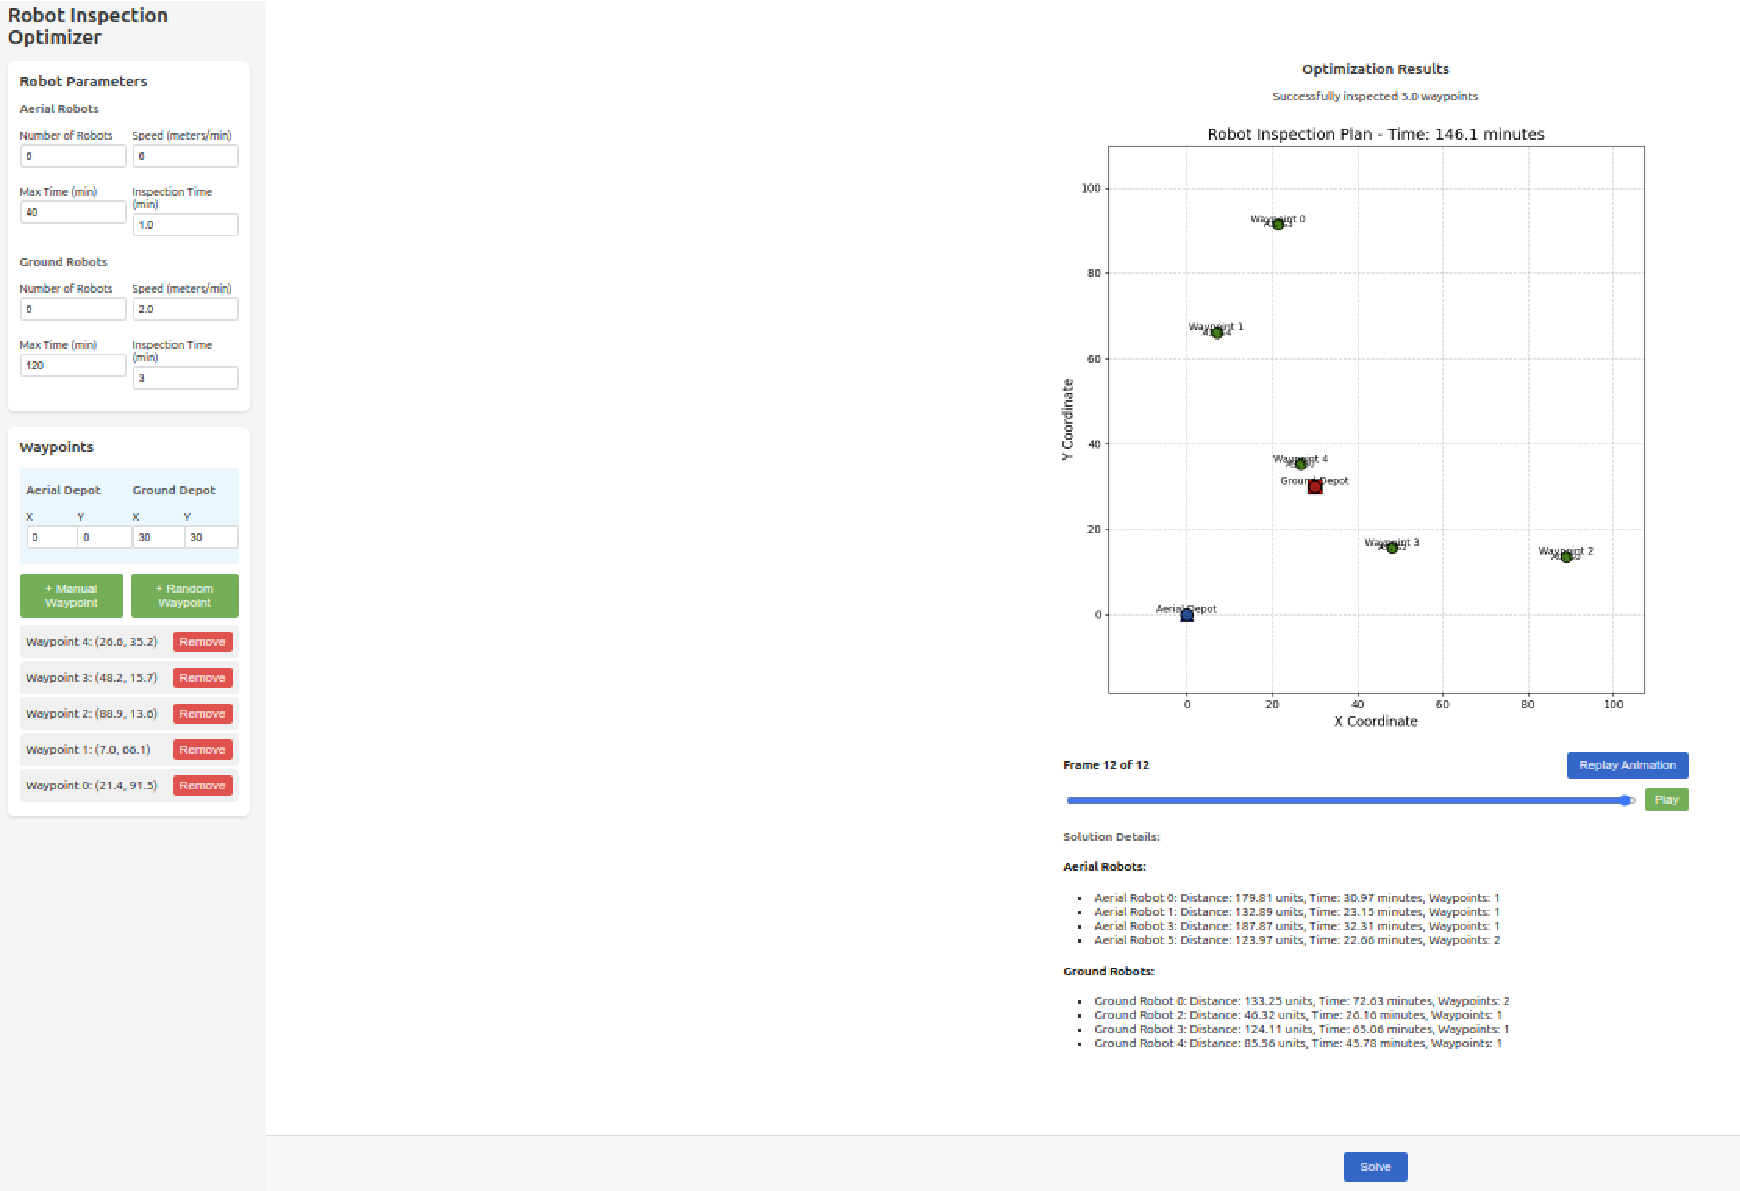
\includegraphics[width=0.9\linewidth,height=0.9\textheight,keepaspectratio]{insp.pdf}
			\caption{Developed browser based GUI showcasing a solved inspection plan.}
			\label{fig:demo}
		\end{figure}


	\section{Numerical Results}\label{numerical_results}




	\section{Conclusion}\label{conclusion}

	In this report a Mixed Integer Linear Program was developed to optimize the inspection coverage of a ground and aerial robot fleet. 
	We formulated a model which maximized the number of waypoints covered by N robots with variable parameters and operating capabilities.
	This formulation was then implemented in a Python program using the PuLP library of solvers and a browser based GUI was developed to allow for an interactive demonstration environment.

	\newpage
	\bibliographystyle{IEEEtran}
	\nocite{*}
	\bibliography{/project/src/ref}

\end{document}